\subsection{CICDDos2019}

\subsubsection{Descripción}

CICDDos2019 es un dataset creado por el Canadian Institute for Cybersecurity que contiene trazas de dos días en los que aparece tráfico benigno y serie de ataques DDoS típicos. \cite{cicddos2019web}. En este se contienen trazas de red en formato pcap y csvs con estadísticas de los flujos generados a partir de CICFlowMeter y posteriormente etiquetados. Para poder ofrecer un dataset público, realista y, además de mantener la privacidad de las comunicaciones originales, se generó tráfico sintético modelado a partir del comportamiento real de los usuarios. En las referencias se menciona el sistema utilizado para generar el comportamiento lo más natural posible de 25 usuarios haciendo uso de HTTP, HTTPS, FTP, SSH y protocolos de correo.

Los elementos de la red interna consisten en:

\begin{itemize}
    \item Servidor web con Ubuntu 16.04 (192.168.50.1 en el primer día, 192.168.50.4 en el segundo día)
    \item Firewall con Fortinet (205.174.165.81)
    \item PC con Windows 7 (192.168.50.8 en el primer día, 192.168.50.9 en el segundo día)
    \item PC con Windows Vista (192.168.50.5 en el primer día, 192.168.50.6 en el segundo día)
    \item PC con Windows 8.1 (192.168.50.6 en el primer día, 192.168.50.7 en el segundo día)
    \item PC con Windows 10 (192.168.50.7 en el primer día, 192.168.50.8 en el segundo día)
\end{itemize}

Adicionalmente, se han generado ataques DDoS basados en reflejos (usar un sistema de terceros para amplificar un ataque) y DDoS basado en exploits (tomar ventaja de vulnerabilidades en los protocolos). Según la información disponible \cite{cicddos2019web}, estos consisten en:

\begin{enumerate}
    \item \textbf{MSSQL}: Generado el primer día de 10:53 a 10:42 y el segundo de 11:36 a 11:45
    \item \textbf{SSDP}: Generado el segundo día de 12:27 a 12:37
    \item \textbf{DNS}: Generado el segundo día de 10:52 a 11:05
    \item \textbf{LDAP}: Generado el primer día de 10:21 a 10:30 y el segundo de 11:22 a 11:32
    \item \textbf{NetBIOS}: Generado el primer día de 10:00 a 10:09 y el segundo de 11:50 a 12:00
    \item \textbf{SNMP}: Generado el segundo día de 12:12 a 12:23
    \item \textbf{PortMap}: Generado el primer día de 9:43 a 9:51
    \item \textbf{WebDDoS}: Generado el segundo día de 13:18 a 13:29
    \item \textbf{NTP}: Generado el segundo día de 10:35 a 10:45
    \item \textbf{TFTP}: Generado el segundo día de 13:35 a 17:15
    \item \textbf{SYN Flood}: Generado el primer día de 11:28 a 17:35 y segundo día de 13:29 a 13:34
    \item \textbf{UDP Flood}: Generado el primer día de 10:53 a 11:03 y segundo día de 12:45 a 13:09
    \item \textbf{UDP-Lag}: Generado el primer día de 11:14 a 11:24 y segundo día de 13:11 a 13:15
\end{enumerate}

\subsubsection{Contenidos csvs}

El conjunto de datos procesados utilizando CICFlowMeter y etiquetado está compuesto por una lista de archivos por cada uno de los dos días en los que se generaron datos, el 3 de noviembre de 2018 y el 1 de diciembre de 2018. Las características ofrecidas son las mismas que las mencionadas en la herramienta CICFlowMeter. En todas las filas existen valores con excepción de algunas en la columna "Flow Bytes/s". Los scripts utilizados para la extracción y representación de los datos son \texttt{extract\_info\_cicddos\_2019.py} y \texttt{plot\_info\_cicddos\_2019.py} disponibles en TODO DEFINIR.

Como podemos ver en las figuras \ref{fig:cicddos_2019_csv_03-11_file_results} y \ref{fig:cicddos_2019_csv_01-12_file_results}, los archivos no contienen únicamente ataques etiquetados con su mismo nombre y benignos, sino que algunos contienen entre uno y dos adicionales. Para el primero, las categorías adicionales provienen de otros archivos. Para el segundo, la categoría adicional en UDPLag.csv no tiene ningún archivo específico y su magnitud es de las más bajas. A pesar de esto, si miramos las líneas temporales respectivas en las figuras \ref{fig:cicddos_2019_csv_03-11_timeline} y \ref{fig:cicddos_2019_csv_01-12_timeline}, podemos ver que el único caso donde existen solapamientos es en el caso de WebDDoS y UDP-Lag. Cabe notar que el tráfico benigno se encuentra infrarepresentado, cosa que es posible que no se corresponda con un entorno real, donde el tráfico sea normalmente benigno y los ataques sean relativamente raros e inesperados.

\begin{figure}[!htb]
    \minipage{0.49\textwidth}
      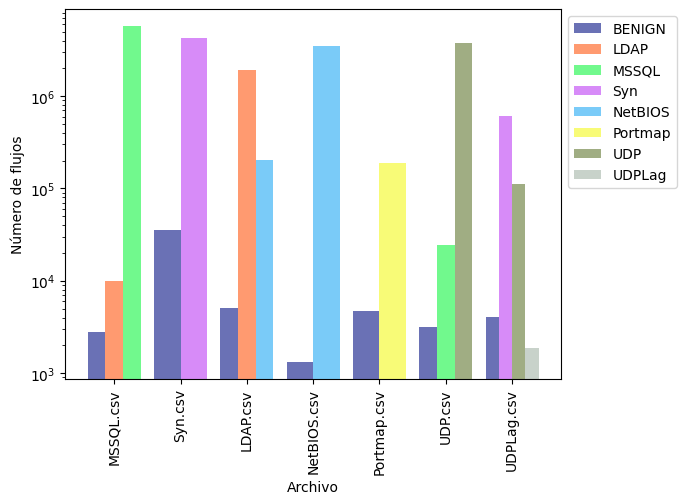
\includegraphics[width=\linewidth]{media/cicddos_2019_csv_03-11_file_results.png}
      \captionsetup{justification=centering}
      \caption{Número de flujos por archivo de las trazas de noviembre 3}\label{fig:cicddos_2019_csv_03-11_file_results}
    \endminipage\hfill
    \minipage{0.49\textwidth}
      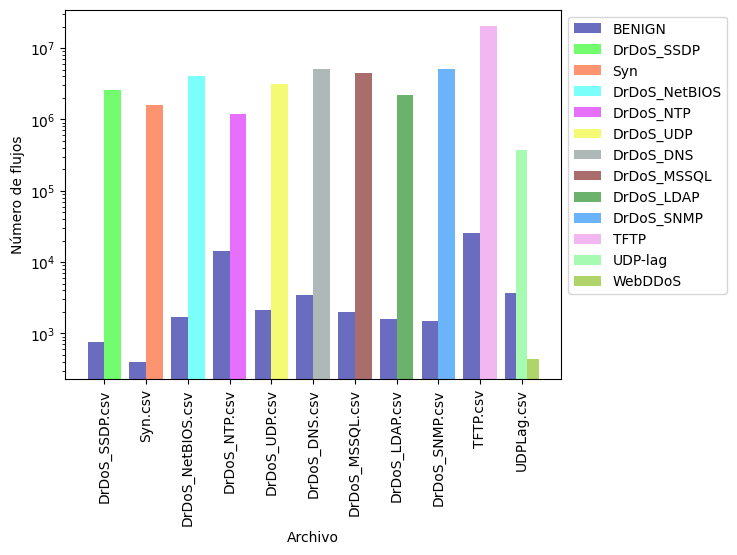
\includegraphics[width=\linewidth]{media/cicddos_2019_csv_01-12_file_results.png}
      \captionsetup{justification=centering}
      \caption{Número de flujos por archivo de las trazas de diciembre 1}\label{fig:cicddos_2019_csv_01-12_file_results}
    \endminipage\hfill
\end{figure}

\begin{figure}[!htb]
    \begin{center}
        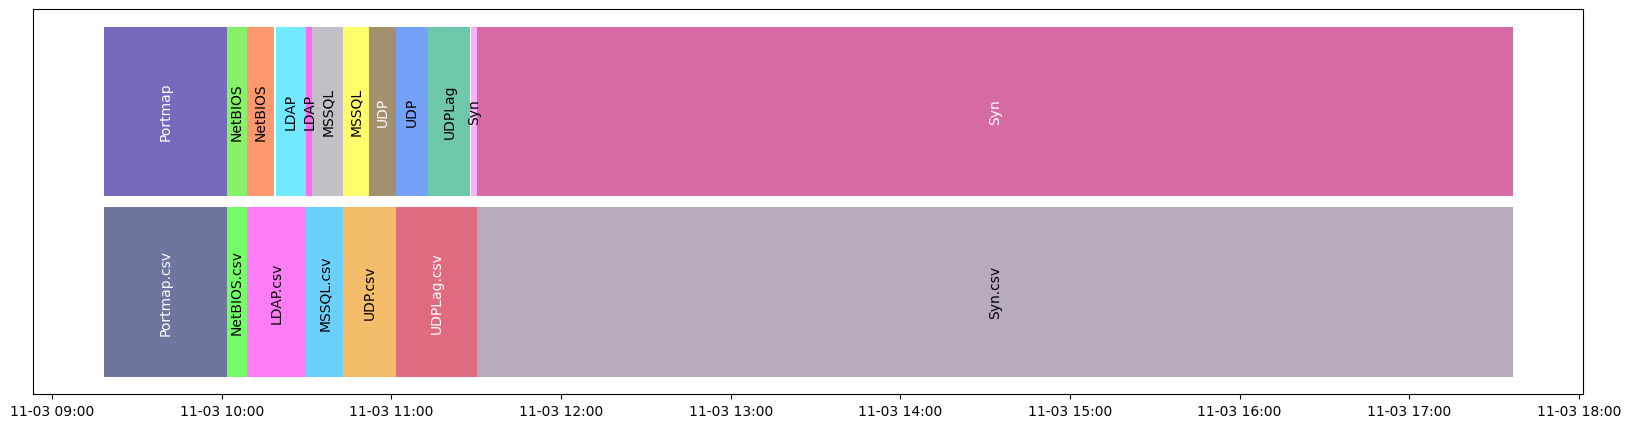
\includegraphics[width=1\linewidth]{media/cicddos_2019_csv_03-11_timeline.png}
    \end{center}
    \captionsetup{justification=centering}
    \caption{Línea temporal de las trazas de noviembre 3 con los archivos (debajo) y los rangos de ataques en estos (arriba)}\label{fig:cicddos_2019_csv_03-11_timeline}
\end{figure}
\begin{figure}[!htb]
    \begin{center}
        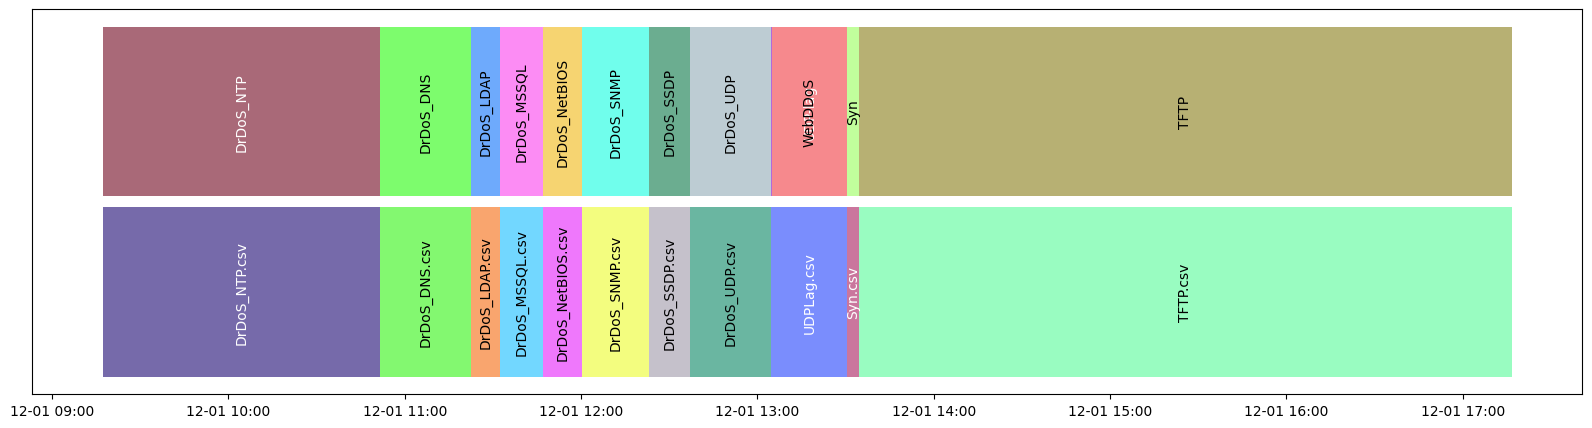
\includegraphics[width=1\linewidth]{media/cicddos_2019_csv_01-12_timeline.png}
    \end{center}
    \captionsetup{justification=centering}
    \caption{Línea temporal de las trazas de diciembre 1 con los archivos (debajo) y los rangos de ataques en estos (arriba)}\label{fig:cicddos_2019_csv_01-12_timeline}
\end{figure}

%\begin{figure}[!htb]
%    \minipage{1\textwidth}
%      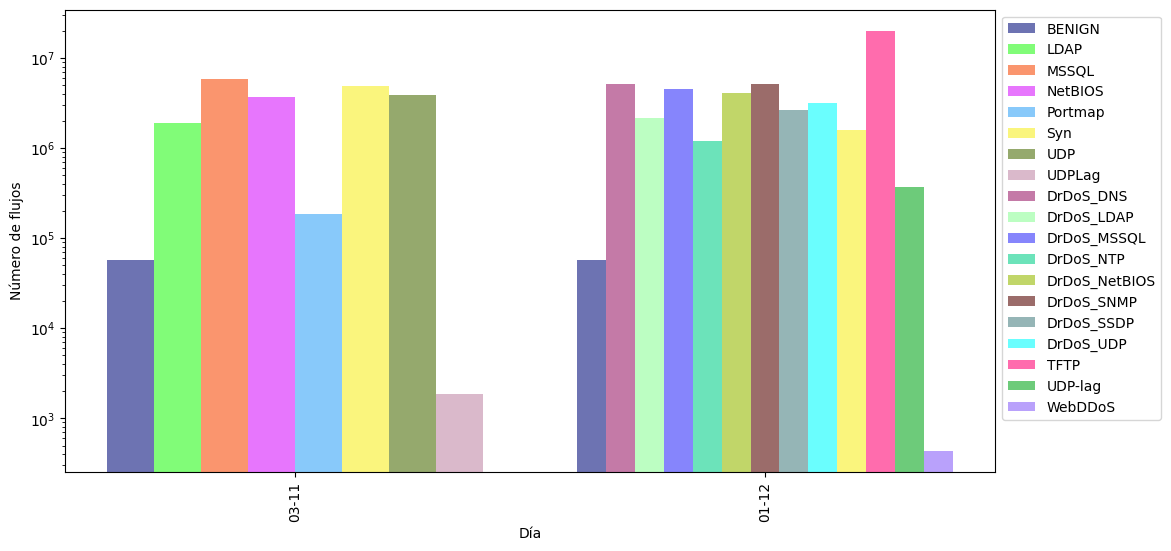
\includegraphics[width=\linewidth]{media/cicddos_2019_csv_day_results.png}
%      \captionsetup{justification=centering}
%      \caption{Número de flujos por archivo de las trazas de noviembre 3}\label{fig:cicddos_2019_csv_day_results}
%    \endminipage
%\end{figure}

\subsubsection{Contenidos pcaps}

El dataset CICDDos2019 ofrece un conjunto de trazas de red de los dos días en los que se generaron datos. Para el primer día (3 de noviembre), hay 145 archivos de unos 190.7 MiB cada uno y un último de 66.5 MiB. Para el segundo día (1 de diciembre), se ofrecen 818 archivos de 190.7 MiB cada uno y uno adicional de 3.7 MiB. En ambos casos, si intentamos abrir el último paquete con Wireshark o generamos cualquier análisis a través de tshark, se nos notifica que el paquete se encuentra 'cortado'. Esto es quizá causado porque, en el momento de generar las trazas, se cortó el proceso de captura precipitadamente. Los scripts utilizados para la extracción de datos es \texttt{extract\_info\_cicddos\_2019\_pcaps\_tshark.sh} y el utilizado para la representacion de estos es \texttt{evaluate\_info\_cicddos\_2019\_pcaps\_tshark.py} disponibles en TODO DEFINIR.

En los pcap, aparecen más direcciones IP en la red del testbed (192.\-168.\-50.\-0/24) de las mencionadas en la información ofrecida en la web del dataset. Concretamente, tenemos que en el primer día aparecen adicionalmente 192.\-168.\-50.\-4, 192.\-168.\-50.\-9 192.\-168.\-50.\-253 y 192.\-168.\-50.\-254. En el segundo día, tenemos que aparecen 192.\-168.\-50.\-253 y 192.\-168.\-50.\-254 además del posible router con IP 192.\-168.\-50.\-1. Adicionalmente, en ambos casos aparece la IP de broadcast (192.\-168.\-50.\-255). Respecto al número de direcciones IP únicas, podemos ver que en el primer día aparecen 1321 y en el segundo 640, teniendo en total 1723 únicas en el transcurso de los dos días. 

Se han generado histogramas con la distribución de la duración de los flujos, número de tramas y número de bytes para poder compararlos con los futuros resultados de la herramienta y comprobar que son consistentes. Como podemos ver en la Figura \ref{fig:cicddos_2019_pcap_duration_distribution}, hay muchos flujos los cuales su duración es relativamente corta y luego hay cierta variedad de flujos de mayor duración. Para el caso de las tramas, podemos observar en la Figura \ref{fig:cicddos_2019_pcap_frames_distribution} que en su mayoría se concentran entre 1 y 1000 tramas y a continuación se reduce drásticamente la cantidad, aunque hay un grupo de flujos los cuales se comprenden entre 10 000 y 100 000. En la Figura \ref{fig:cicddos_2019_pcap_bytes_distribution}, podemos ver que tenemos un caso similar, la mayoría se concentra en las partes bajas, después decrece y hay un grupo numeroso separado el cual realiza una gran transferencia de datos.

\begin{figure}[H]
    \begin{center}
        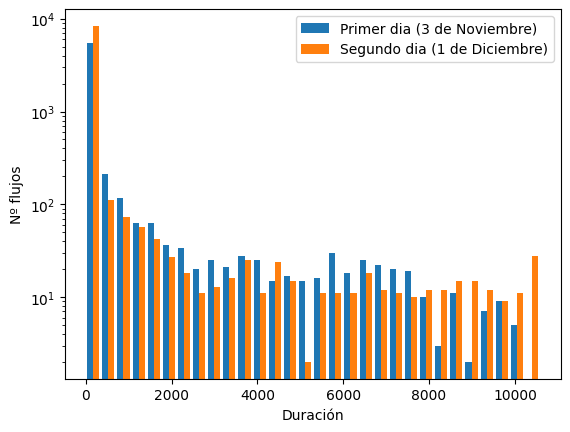
\includegraphics[width=0.49\linewidth]{media/cicddos_2019_pcap_duration_distribution.png}
    \end{center}
    \captionsetup{justification=centering}
    \caption{Distribución duraciones de flujos en CICDDos2019}\label{fig:cicddos_2019_pcap_duration_distribution}
\end{figure}

\begin{figure}[H]
    \minipage{0.49\textwidth}
      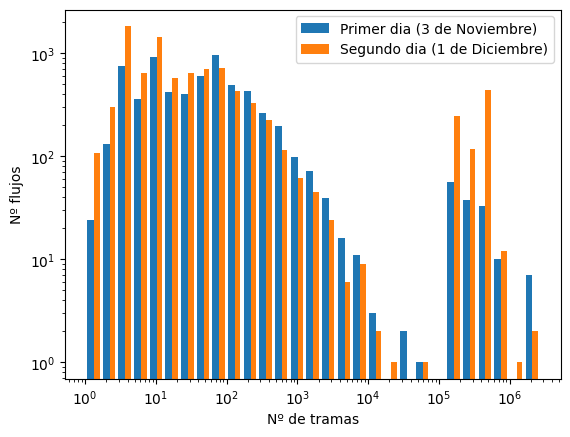
\includegraphics[width=\linewidth]{media/cicddos_2019_pcap_frames_distribution.png}
      \captionsetup{justification=centering}
      \caption{Distribución número de tramas en flujos en CICDDos2019}\label{fig:cicddos_2019_pcap_frames_distribution}
    \endminipage\hfill
    \minipage{0.49\textwidth}
      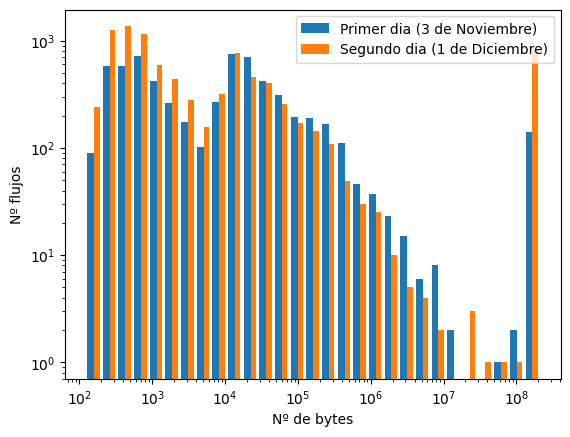
\includegraphics[width=\linewidth]{media/cicddos_2019_pcap_bytes_distribution.png}
      \captionsetup{justification=centering}
      \caption{Distribución número de bytes en flujos en CICDDos2019}\label{fig:cicddos_2019_pcap_bytes_distribution}
    \endminipage\hfill
\end{figure}

En la tabla \ref{table:cicddos2019protocolsip} podemos ver el resultado del análisis con tshark sobre la repartición de los diferentes protocolos de transporte sobre IPv4. Como podemos ver, nos indica que la mayoría (77.5\%) de los datos van sobre UDP y el resto se encuentra principalmente repartido entre protocolos que no ha podido identificar (14.26\%) y TCP (8.21\%). Adicionalmente, podemos observar que existen algunas tramas residuales de otros protocolos (SCTP, IBQP e IPX).

%Generated with /workspaces/tfg/scripts/evaluate_info_cicddos_2019_pcaps_tshark.py
\begin{table}[H]
    \begin{center}
        \begin{tabular}{|c | c c|} 
            \hline
            \textbf{Protocolo} & \textbf{Nº Tramas} & \textbf{Porcentaje}\\
            \hline\hline
IP & 3.12e+08 & 100.000 \\
UDP & 2.42e+08 & 77.509 \\
NONE & 4.46e+07 & 14.275 \\
TCP & 2.56e+07 & 8.212 \\
SCTP & 4.19e+03 & 0.001 \\
IBQP & 3.89e+03 & 0.001 \\
IPX & 3.19e+03 & 0.001 \\
            \hline
        \end{tabular}
    \end{center}
    \caption{Protocolos identificados analizando exclusivamente la capa IP en CICDDos2019}
    \label{table:cicddos2019protocolsip}
\end{table}


Si miramos la cantidad de información transmitida por las diferentes capas de red y de transporte en la tabla \ref{table:cicddos2019protocols}, podemos ver cómo la mayor parte del tráfico sigue consistiendo en UDP, TCP y otro no identificado (data). De los 174.8 GiB transmitidos en total, menos de 10 MiB consisten en tráfico no IPv4. Adicionalmente, un 66.01\% de este tráfico es específicamente UDP, haciendo uso de posibles diversos protocolos en la siguiente capa. Es posible que la cantidad de protocolos sea engañosa, ya que es posible que este número haya sido exagerado a causa de ataques de escaneo en el dataset. Los otros dos puestos sobre la capa de red, consisten en 57.1 GiB (32.66\%) que tshark no pudo identificar y 2.2GiB (1.25\%) de tráfico TCP. Cabe notar que en este análisis, los protocolos residuales detectados en la capa de transporte sobre IP son diferentes a los de la tabla \ref{table:cicddos2019protocolsip}.

%Generated with /workspaces/tfg/scripts/evaluate_info_cicddos_2019_pcaps_tshark.py
\begin{table}[H]
    \begin{center}
        \begin{tabular}{|c c c | c c c|} 
            \hline
            \textbf{L0} & \textbf{L1} & \textbf{L2} & \textbf{Tramas} & \textbf{Bytes} & \textbf{Nº subprotocolos}\\
            \hline\hline
eth &- &- & 3.12e+08 & 174.8GiB & 5 \\
eth &ip &- & 3.12e+08 & 174.8GiB & 7 \\
eth &ip &data & 4.44e+07 & 57.1GiB & 0 \\
eth &ip &udp & 2.42e+08 & 115.4GiB & 187 \\
eth &ip &icmp & 2.01e+05 & 29.9MiB & 64 \\
eth &ip &tcp & 2.56e+07 & 2.2GiB & 7 \\
eth &ip &ospf & 4.42e+04 & 4.0MiB & 0 \\
eth &ip &igmp & 1.00e+02 & 5.9KiB & 0 \\
eth &ip &rsvp & 2.00e+00 & 260.0B & 0 \\
eth &llc &- & 3.54e+04 & 3.0MiB & 3 \\
eth &llc &stp & 2.93e+04 & 1.8MiB & 0 \\
eth &llc &dtp & 3.90e+03 & 228.8KiB & 0 \\
eth &llc &cdp & 2.17e+03 & 977.2KiB & 0 \\
eth &ipv6 &- & 2.00e+04 & 2.9MiB & 2 \\
eth &ipv6 &udp & 1.54e+04 & 2.5MiB & 5 \\
eth &ipv6 &icmpv6 & 4.59e+03 & 418.5KiB & 0 \\
eth &arp &- & 9.14e+03 & 535.6KiB & 0 \\
eth &lldp &- & 1.22e+02 & 7.1KiB & 0 \\
            \hline
        \end{tabular}
    \end{center}
    \caption{Primeras tres capas de protocolos identificados en CICDDos2019}
    \label{table:cicddos2019protocols}
\end{table}


Finalmente, si abrimos la primera traza de red del primer día de captura, podemos ver que en la capa de enlace aparecen dos estándares: 'Ethernet II' como podemos ver en la figura \ref{fig:cicddos_2019_pcap_03-11_0_ethii_packet} y 'IEEE 802.3 Ethernet' en la figura \ref{fig:cicddos_2019_pcap_03-11_0_llc_packet}. Ambos estándares son similares, la principal diferencia entre ellos es parte de la estructura de la trama \cite{IBMeth2vsllc}. Se puede observar que la mayoría de paquetes que utilizan IP para la capa de red, utilizan el primero como capa de enlace. Los casos donde aparece el segundo parece principalmente ser en casos de comunicación interna entre routers.

\begin{figure}[H]
    \minipage{0.49\textwidth}
      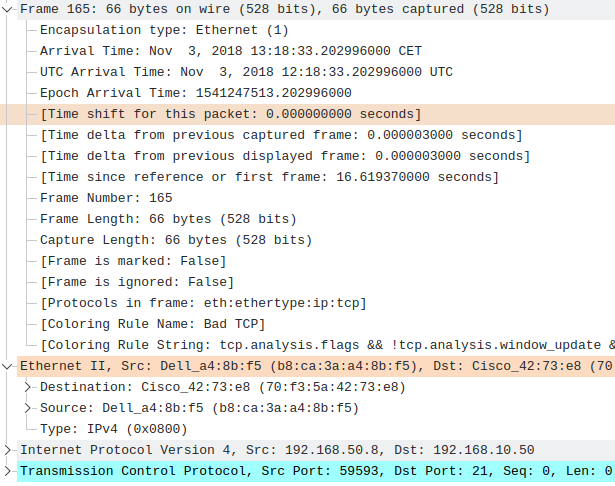
\includegraphics[width=\linewidth]{media/cicddos_2019_pcap_03-11_0_ethii_packet.png}
      \captionsetup{justification=centering}
      \caption{Paquete EthII en CICDDos2019}\label{fig:cicddos_2019_pcap_03-11_0_ethii_packet}
    \endminipage\hfill
    \minipage{0.49\textwidth}
      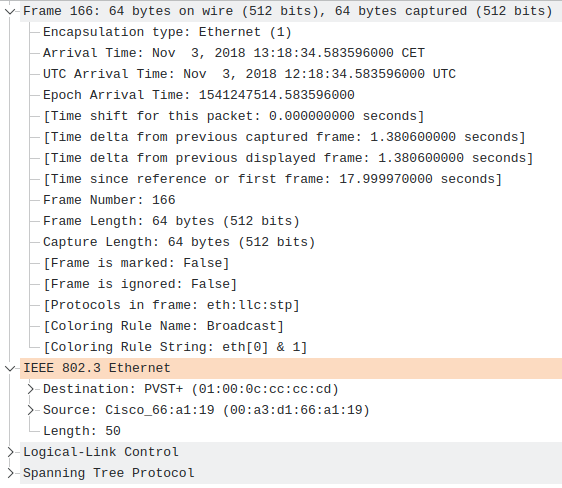
\includegraphics[width=\linewidth]{media/cicddos_2019_pcap_03-11_0_llc_packet.png}
      \captionsetup{justification=centering}
      \caption{Paquete LLC en CICDDos2019}\label{fig:cicddos_2019_pcap_03-11_0_llc_packet}
    \endminipage\hfill
\end{figure}
